\documentclass[11pt,twocolumn]{article}
\usepackage{graphicx}
\usepackage[italian]{babel}
\usepackage{url}

\title{{\textbf{Il lessico della Costituzione nel suo farsi. \\ 
Creazione e analisi di un corpus dell'Assemblea Parlamentare}}.}
\author{
  Greta Gorzoni \\
  \texttt{greta.gorzoni@studio.unibo.it}  \\
  0001122966 }
\date{}

\begin{document}

\maketitle

\section{Introduzione}
L'Assemblea Costituente è eletta il 2 giugno del 1946. Nell'arco del 1947 ha il compito di discutere il testo della Costituzione. Il dibattito che si sviluppa nelle relazioni dei costituenti è ciò che plasma il testo costituzionale e dove è possibile ricercare la preminenza e la rilevanza dei temi maggiormente dibattuti.
Il presente progetto mira a sviluppare una modalità di analisi interdisciplinare che si possa applicare alle fonti storiche di questo tipo. L'obiettivo del progetto è quello di esplorare il lessico e i temi prevalenti nei discorsi dei membri dell'Assemblea, utilizzando tecniche di elaborazione del linguaggio naturale (NLP) e Topic Modelling. L'analisi è stata realizzata tramite un flusso di lavoro che include la creazione del corpus, la pre-elaborazione dei dati, l'applicazione di modelli statistico-frequenziali e, infine, l'uso di tecniche di Topic Modelling per identificare e visualizzare i principali temi trattati nel dibattito costituente. Il lavoro di programmazione è stato realizzato principalmente con l'ausilio delle librerie Python \textit{BeautifullSoup}, \textit{spaCy}, \textit{Plotly}, \textit{Gensim}, e \textit{pyLDAvis}.

\section{Costruzione del Corpus}
\subsection {Web scraping}
Le relazioni dell'Assemblea Costituente sono disponibili nella banca dati della Camera dei Deputati. 
Per raccogliere il materiale testuale di ciascuna relazione, è stato sviluppato un programma che utilizza tecniche di web scraping. È stato estratto il testo da ogni documento, raccogliendo anche i metadati rilevanti. Il processo è stato automatizzato, iterando su tutte le pagine del sito e su quelle successive. Il programma, utilizzando la libreria \textit{BeautifulSoup}, estrae i link dei documenti dalle pagine web, li segue per ottenere i contenuti, e salva i testi in file separati. Ogni documento è identificato in base a un nome file che include ID, data della seduta e relatore, per facilitarne la successiva analisi.
\subsection {Regular expressions}
Il testo estratto dalla banca dati era completamente in caratteri maiuscoli e presentava una codifica problematica per quanto riguarda accenti e apostrofi. Per correggere queste anomalie, sono state applicate espressioni regolari al fine di normalizzare il testo e renderlo leggibile per la successiva elaborazione con la libreria \textit{spaCy}.
\section{Analisi}

\subsection {Statistico/frequenziale}

Il primo proposito di analisi è stato quello di far emergere le parole maggiormente utilizzate nel dibattito. Per evidenziare le parole più frequenti all'interno del corpus era fondamentale isolare le parole semanticamente piene, onde evitare che, per la legge di Zipf, emergessero come più frequenti le parole grammaticali. Dopo aver effettuato sul testo tokenizzazione e pos-tagging, piuttosto che escludere solo una lista precompilata di stop words, si è preferito filtrare il pos-tag delle parole, evidenziando le più frequenti tra: nomi, aggettivi, verbi e avverbi. 

Sebbene, da un punto di vista teorico, è noto quanto poco accordo vi sia nella classificazione in categorie lessicali e quanto sia complesso distinguere in alcuni casi significato lessicale e grammaticale,  sul piano computazionale la risorsa WordNet composta da quattro database per le categorie sopracitate di nomi, aggettivi, verbi e avverbi e la libreria \textit{NLTK} ci pongono in continuità con una solida riflessione già ampiamente percorsa nel trovare una soluzione pratica per ricercare il significato lessicale isolando queste categorie. Sono stati esclusi inoltre gli ausiliari essere/avere e gli avverbi con principali funzioni grammaticali. 

\begin{figure}

    \centering
    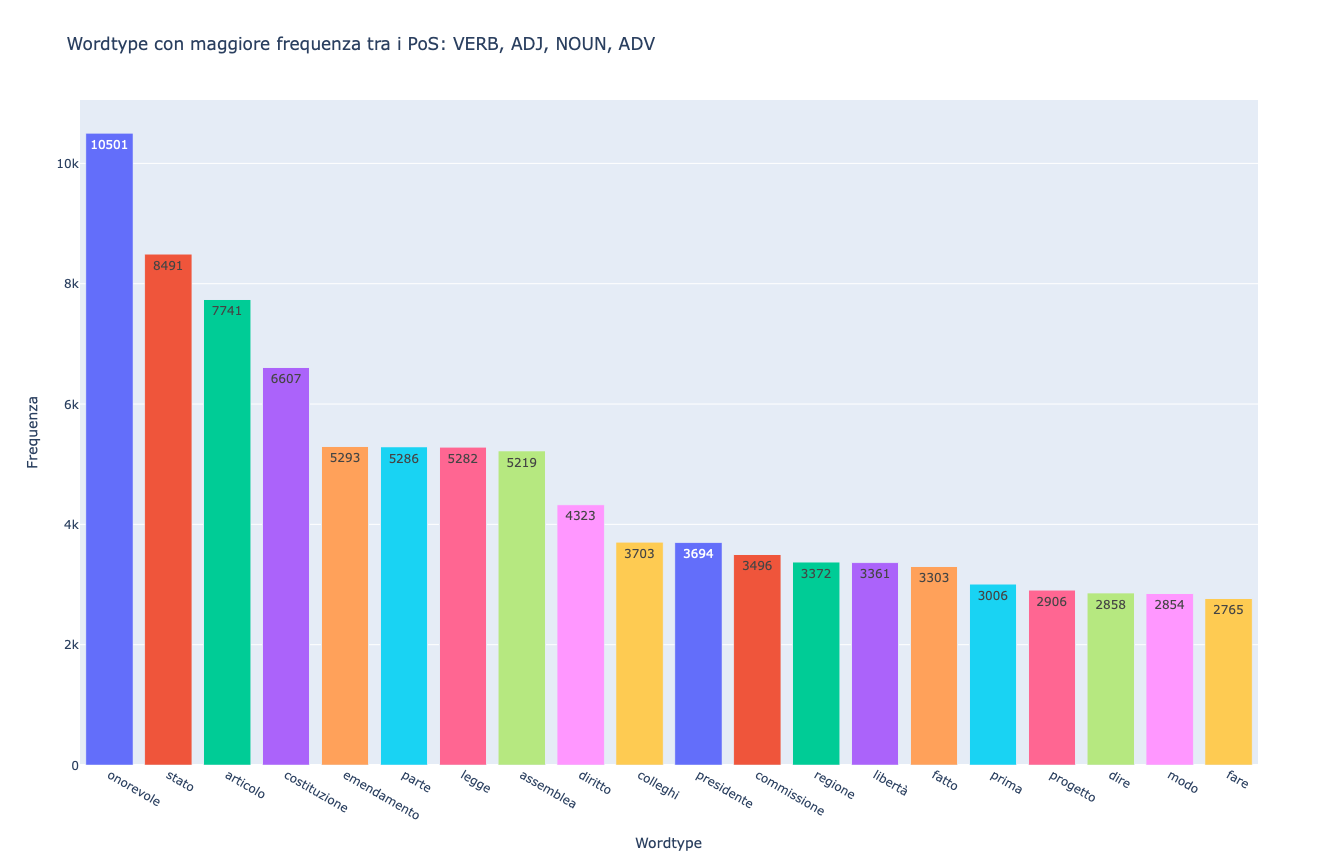
\includegraphics[width=0.9\linewidth]{newplot.png}
    \caption{20 parole più frequenti nel corpus}
    \label{fig:enter-label}
\end{figure}

È stato utilizzato un oggetto \textit{Counter} per registrare la frequenza di ciascun token, permettendo di determinare le 20 parole più frequenti. I dati sono stati poi organizzati in un data set utilizzando la libreria \textit{pandas}. Per la visualizzazione, è stato generato un grafico interattivo a barre tramite \textit{Plotly}, che è stato salvato in formato \textit{HTML} permettendo la visualizzazione delle frequenze lessicali, come mostra la Figura 1.

Dalle parole più frequenti in assoluto l'analisi si è spostata verso la ricerca del lessico specifico del sottocodice linguistico in analisi. Quindi, non semplicemente le parole con il maggior numero di occorrenze, ma le parole particolarmente rappresentative di un sub-corpus, mediando tra le occorrenze nel sup-corpus (valorizzandole) e le occorrenze nel corpus complessivo (penalizzandole). Per fare ciò si è utilizzata la metrica \textit{TF-IDF} (Term Frequency-Inverse Document Frequency). 

Si è scelto di analizzare l'andamento temporale del discorso parlamentare sulla Costituzione, isolando come sub-corpus le relazioni di ciascun mese. Grazie al precedente lavoro di nominazione dei file attraverso metadati, è stato possibile estrarre per ogni relazione il mese in cui è stata pronunciata. Tale funzione è stata integrata nell'iterazione della processazione del testo di ogni file, al fine di avere in output un dizionario dove ogni \textit{key} corrispondesse ai mesi e ogni rispettivo \textit{value} comprendesse le relazioni pronunciate in quel mese. L'oggetto dizionario è stato trasformato in una lista di stringhe, come richiesto in input dalla funzione \textit{tfidfVectorizer.fit\_transform} di \textit{sklearn}, per ottenere una rappresentazione dei dati in matrice delle parole e dei relativi valori TF-IDF. Utilizzando l'indicizzazione della matrice sono state estratte le parole con valore maggiore di TF-IDF per ciascun mese.
Per la visualizzazione, è stato generato un grafico interattivo tramite Plotly, con la disposizione circolare dei mesi, che è stato salvato in formato HTML. Con il parametro hovertemplate in \textit{plotly.graph\_objects.Scatter} si è resa interattiva la visualizzazione del grafico, mostrando con il passaggio del mouse da parte dell'utente le relative parole specifiche di quel mese, come mostra la Figura 2.
\begin{figure}
    \centering
    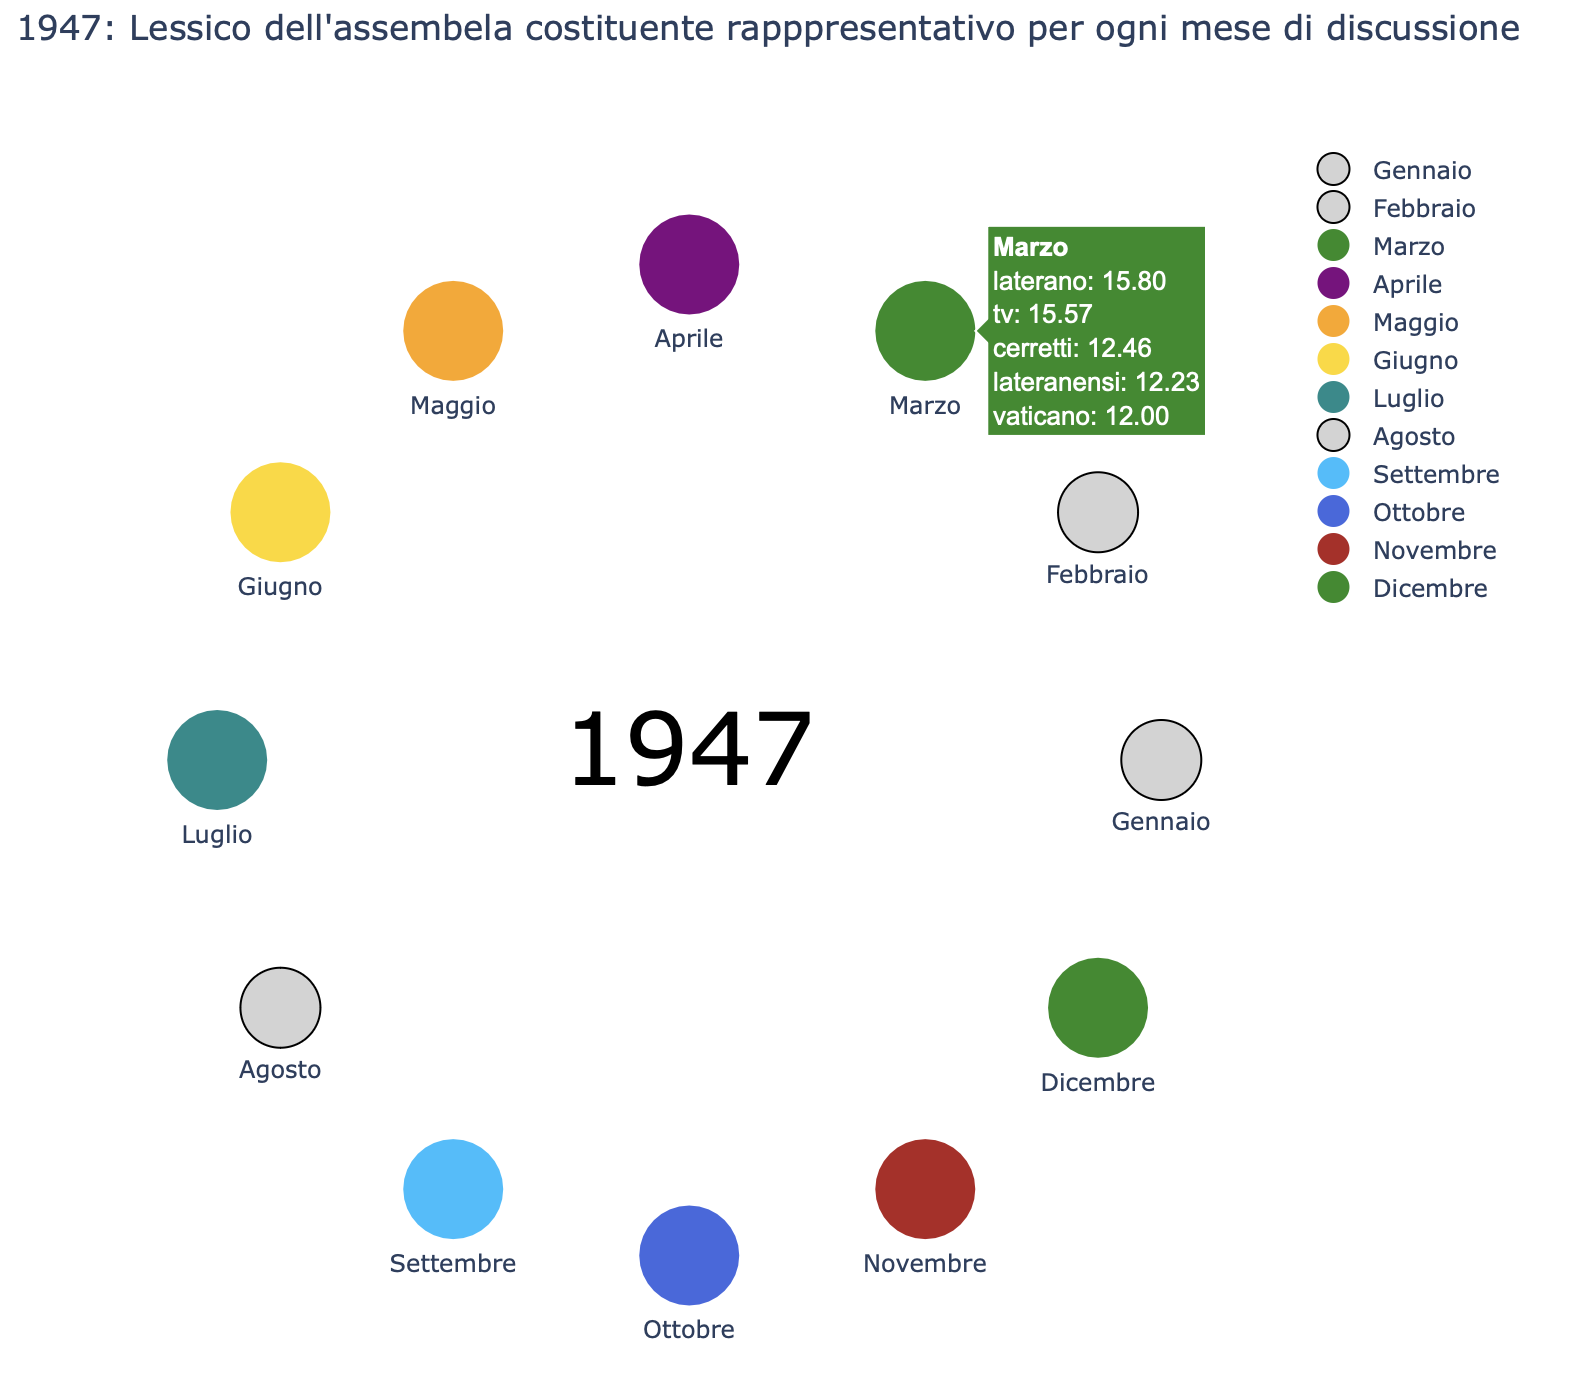
\includegraphics[width=0.5\linewidth]{TF_IDF.png}
    \caption{Parole specifiche, metrica TF-IDF}
    \label{fig:enter-label}
\end{figure}

\subsection{Topic Modelling}

Nel proposito di indagare non solo il lessico della discussione costituzionale, ma le relazioni che si instaurano nel lessico, si è indagato il corpus attraverso Topic Model, che permette l'individuazione automatica dei principali argomenti in un corpus documentale. Un tema è rappresentato da un set di token, che osservati nell'insieme suggeriscono il tema comune di cui sono espressione. Il task consiste nell'individuare i topic del corpus e poter poi analizzare quanto ciascun topic sia rilevante per ogni singola relazione di cui il corpus si compone. 

\subsubsection{Modello}
Il testo è stato pre-processato linguisticamente con la libreria \textit{spaCy} e di ogni token è stata considerata la forma del suo lemma, per evitare di avere token diversi dal punto di vista della flessione morfologica, ma che esprimono lo stesso concetto semantico. Per la costruzione del Topic Model, tra i modelli possibili si è scelto di seguire LDA (\textit{Latent Dirichlet Allocation}), implementandolo attraverso la libreria Gensim. Si è generato, con la funzione \textit{gensim.corpora.Dictionary}, un dizionario che associa ogni lemma a un identificativo e conseguentemente ogni documento è stato rappresentato come una \textit{Bag of Words}, secondo il dizionario. Questa tecnica consente di considerare ogni documento come una \textit{lista}, che diventa l'oggetto input della funzione \textit{gensim.models.TfidfModel()}, con cui si attribuisce il peso relativo TF-IDF.
Attraverso il corpus elaborato con TF-IDF e il dizionario si costruisce un modello LDA. Sono stati scelti 8 topic, con un numero di passaggi pari a 50 e di iterazioni pari a 150. I parametri \textit{alpha} e \textit{eta} sono stati configurati per ottimizzare la distribuzione dei topic all'interno del corpus. Tali parametri, insieme ai passaggi e alle iterazioni, sono stati scelti per bilanciare il tempo di esecuzione con la qualità dei risultati ottenuti. Il parametro eta in particolare è stato fissato a un valore basso come 0.1 per ottenere argomenti con parole chiave ben definite, favorendo l'interpretabilità.

Il modello è stato caricato e  visualizzato con la libreria pyLDAvis. Come mostra la Figura 3, si è così ottenuta un'infografica del Topic Model che presenta i principali argomenti discussi durante l'Assemblea Costituente in Italia, tra marzo e dicembre 1947. Questa visualizzazione fornisce una panoramica visiva che mostra le relazioni tra i temi e le parole chiave che li definiscono, consentendo di esplorare i temi in modo interattivo, evidenziando la distribuzione delle parole e l'importanza di ciascun tema nel contesto del corpus.

\begin{figure}
    \centering
    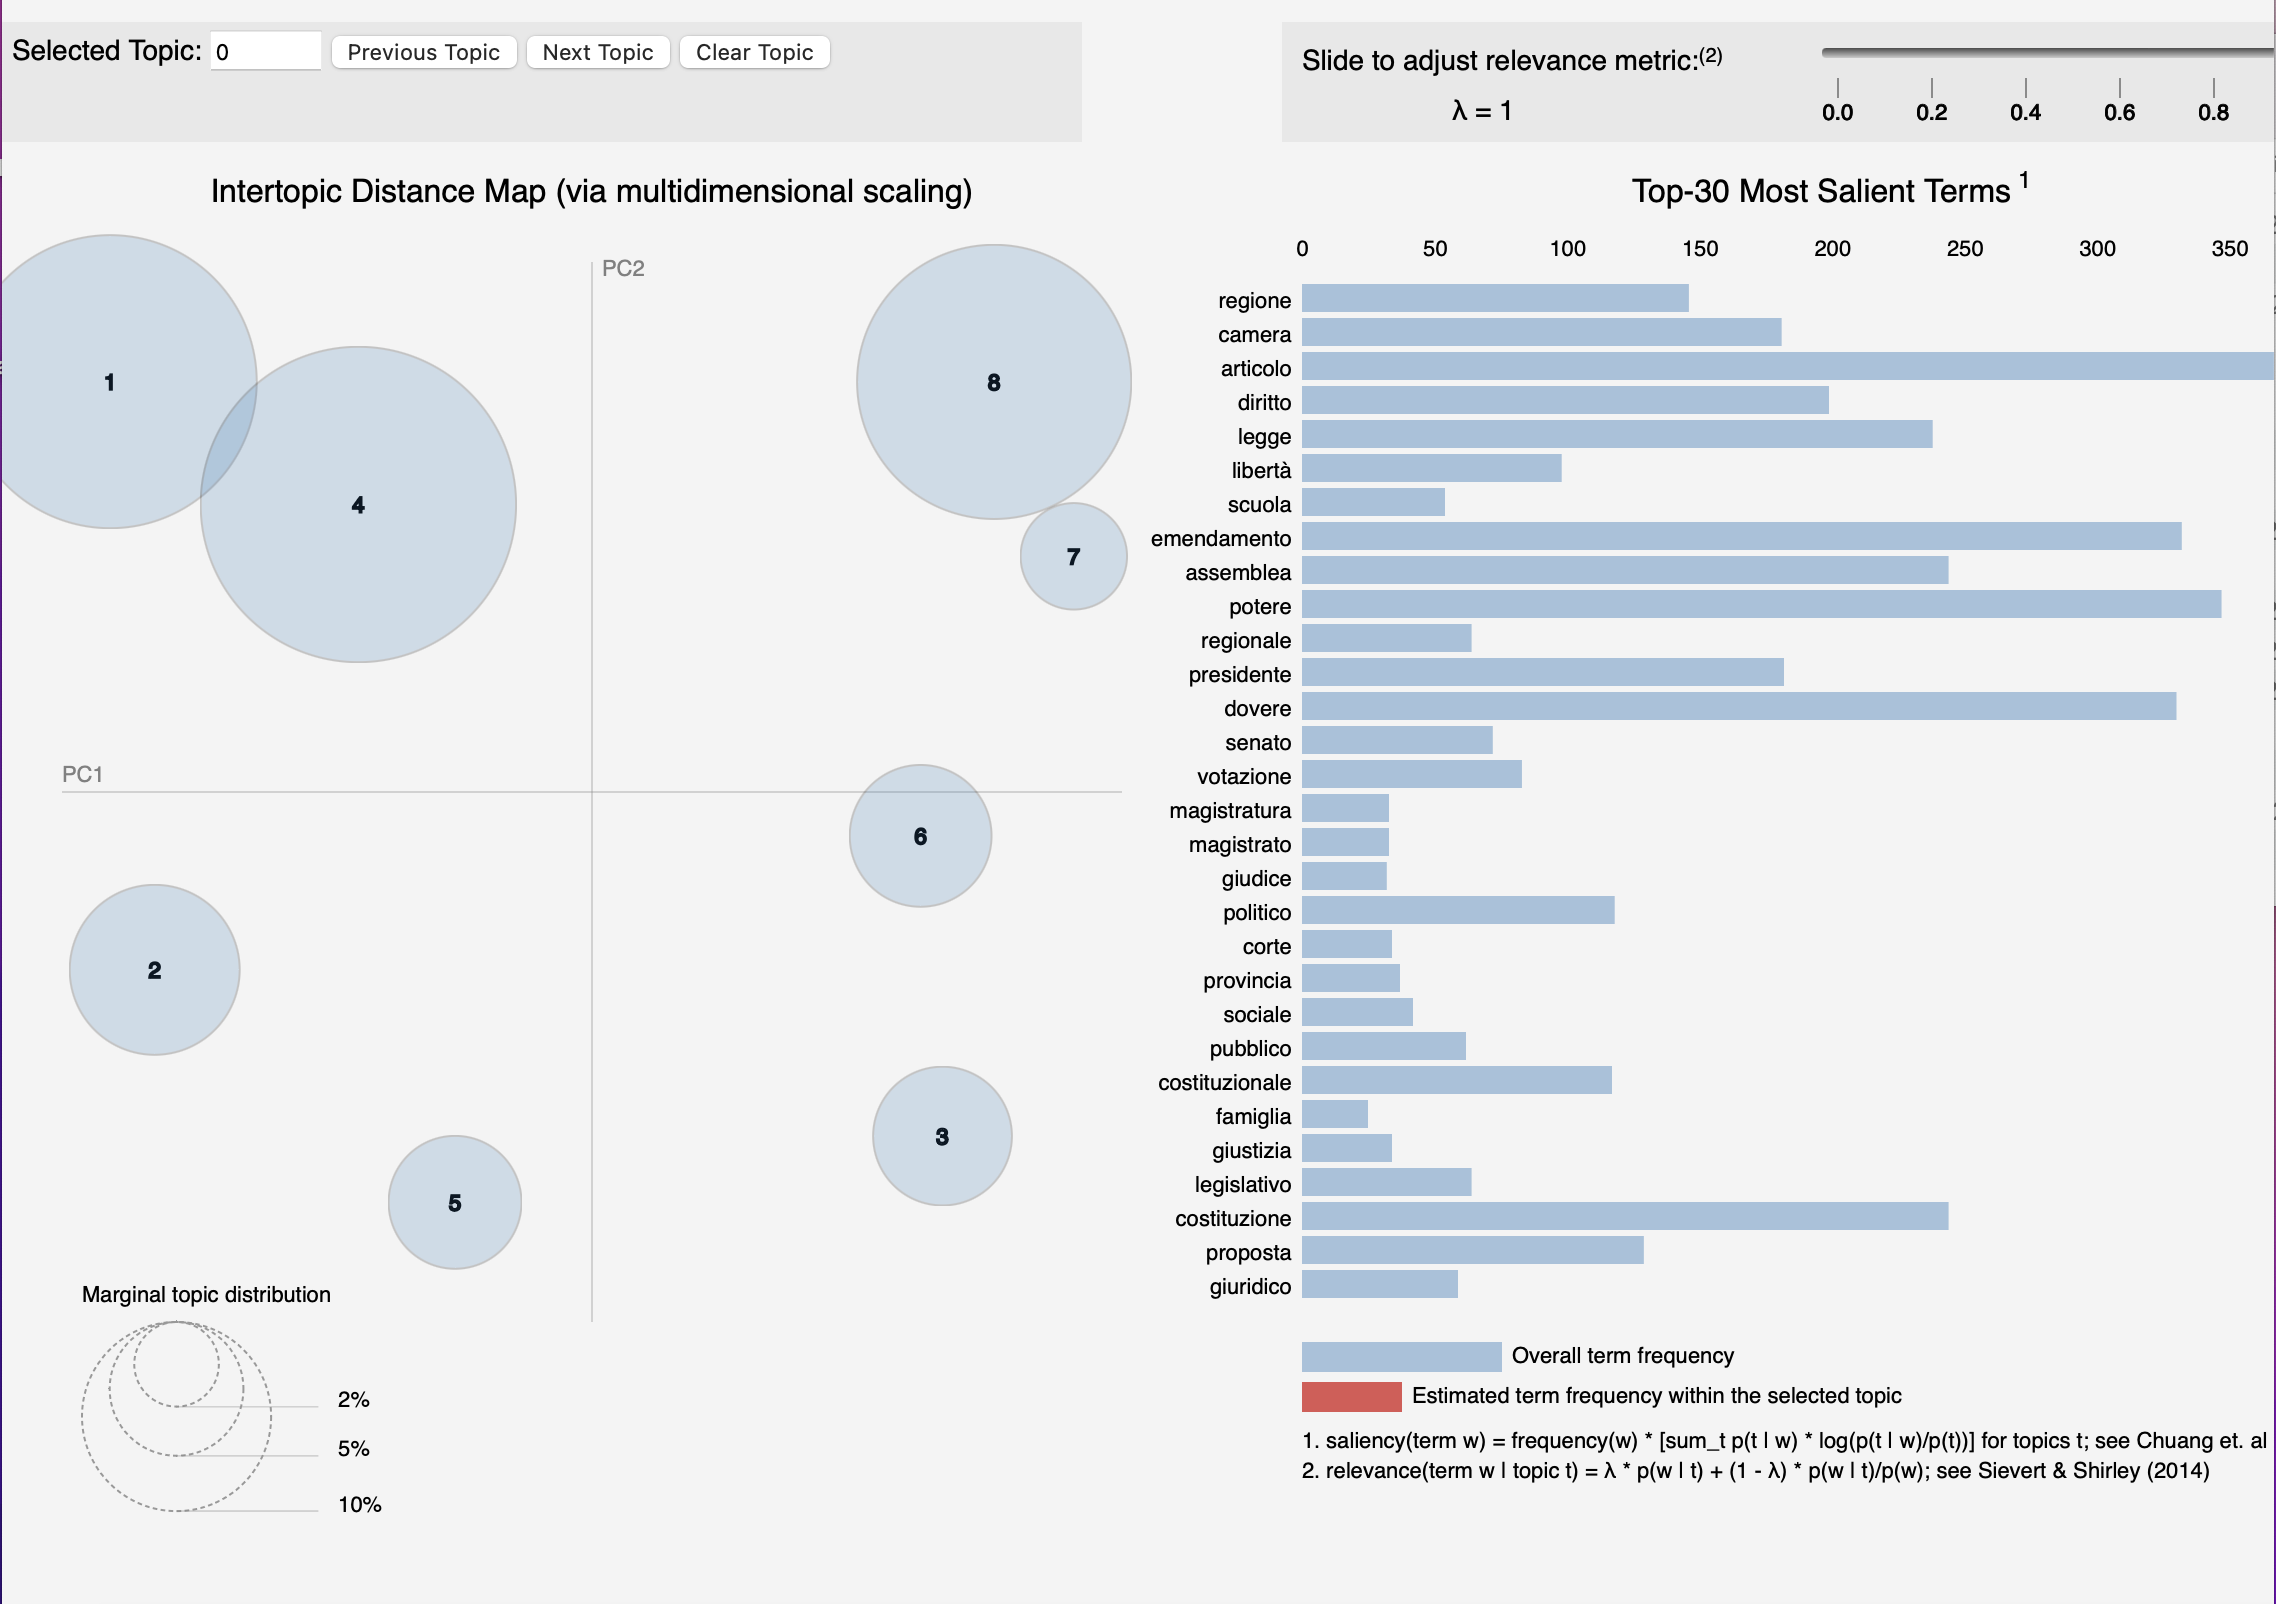
\includegraphics[width=0.9\linewidth]{topic_model.png}
    \caption{Infografica Topic Model}
    \label{fig:enter-label}
\end{figure}

\subsubsection{Analisi documenti}

Si è voluto, in ultima istanza, dedicare una parte del progetto alla valorizzazione dell'interazione con l'utente, attraverso la funzione \textit{input()}. L'analisi della distribuzione probabilistica dei topic nel documento si configura in prima istanza richiedendo di specificare il nome della relazione da analizzare.
Basandosi sul modello LDA precedentemente addestrato sul corpus, viene creata una \textit{Bag of Word} del documento (sul dizionario già creato) e il documento viene quindi analizzato attraverso il modello LDA, generando una distribuzione probabilistica degli argomenti identificati nel testo.

\section{Conclusioni}
Il progetto muove dal proposito di costruire un corpus rappresentativo della discussione dell'Assemblea costituzionale, normalizzarlo e analizzarlo con tecniche di NLP per individuare, attraverso il linguaggio e le sue relazioni semantiche e quantitative, aspetti contenutistici non riscontrabili attraverso analisi impressionistiche. In fase di design, il progetto è stato concepito con una prospettiva interdisciplinare. Gli output interattivi, in formato HTML e realizzati con strumenti come \textit{Plotly}, rappresentano un tentativo di agevolare la comprensione dei dati, contribuendo così a un dialogo più aperto tra discipline diverse. Il progetto si colloca in un panorama di crescente interesse per l'applicazione di NLP nel campo delle fonti storiche. Rispetto a studi simili presenti in letteratura, che spesso si concentrano su corpora più ampi o generici, questo progetto presenta un approccio più specifico e mirato, ma ne emerge anche una vulnerabilità: la capacità dei modelli di identificare pattern semantici profondi è limitata dall'omogeneità del corpus e dalla presenza di formule retoriche convenzionali. 

In questa cornice, il progetto si propone come un tentativo di esplorazione iniziale, che ha messo in luce l'importanza della connessione tra analisi quantitativa e qualitativa e di strumenti computazionali come il Topic Model che la favoriscano. Il Topic Model sul corpus dell'Assemblea Costituzionale ha permesso di scoprire elementi linguistici cruciali per la Costituzione, ma assenti nel testo finale. Questi aspetti sono stati resi visibili grazie all'analisi computazionale, suggerendo nuove prospettive per lo studio delle fonti storiche, che esplorino le strutture linguistiche e tematiche profonde, aprendo a nuove prospettive interpretative basate su evidenze empiriche.

\newpage

\section{\textbf{Bibliografia}}
\begin{itemize}

\item {BeautifulSoup documentation}: \url{https://www.crummy.com/software/BeautifulSoup/bs4/doc/}
\item {spaCy documentation}: 
\url{https://spacy.io/api/doc}
\item {Plotly documentation}: 
\url{https://plotly.com/python/}
\item {Gensim documentation}: 
\url{https://radimrehurek.com/gensim/auto_examples/index.html#documentation}
\item {pLDAvis documentation}: 
\url{https://pyldavis.readthedocs.io/en/latest/index.htm}
\item {Topic Modeling with Gensim}:
\url{https://www.machinelearningplus.com/nlp/topic-modeling-gensim-python/#18dominanttopicineachsentence}


\end{itemize}
\end{document}